\subsection{Implementation}
\label{sec:solution:impl}

We will describe the implementation of some of the more important parts of the
KudOS file server in this section, approximately in order from userspace toward
the disk. We will also describe the online configuration mechanism, and the
userspace tools that make use of it. Figure~\ref{fig:loc} shows the relative
sizes of various modules in the system, in lines of code.

\begin{figure}[htb]
\begin{center}
  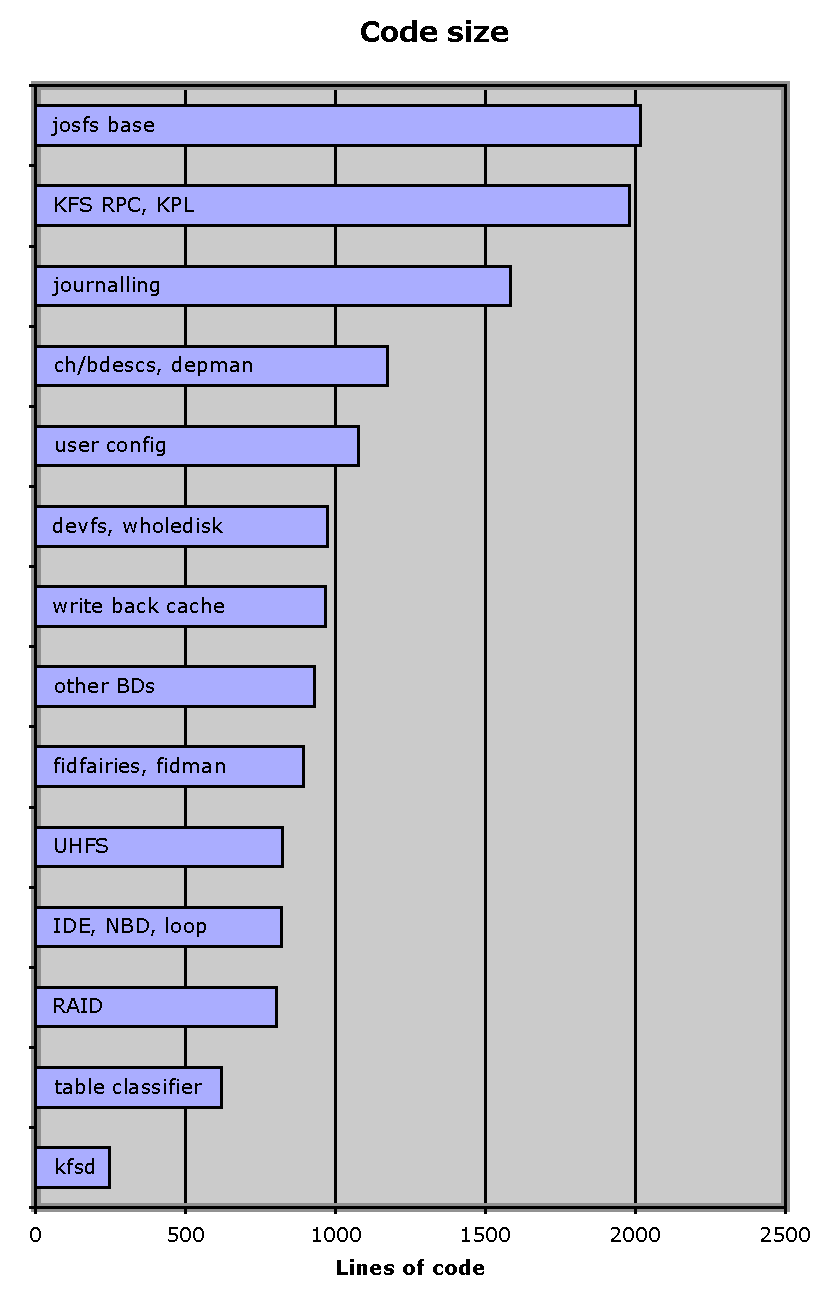
\includegraphics[width=8.1cm]{loc_graph}
  \caption{Lines of Code for Various Modules}
  \label{fig:loc}
\end{center}
\end{figure}

\subsubsection{KPL}
\label{sec:solution:impl:kpl}

The KudOS Presentation Layer (KPL) integrates the user level file descriptor
interface with the CFS interface. Many file system functions are mapped directly
from KPL to CFS, but some require some extra work. For example, the stat()
function uses CFS's get\_metadata() function to get the data to return.
Additionally, KPL provides the authorization tokens to fidprotector.

This allows existing user programs to call into this file server in the same way
they called into the original file server. User programs can be switched back to
use the original file server by changing only a small set of wrapper functions
which call either the new KPL functions or the original functions.

\subsubsection{UHFS}
\label{sec:solution:impl:uhfs}

If the CFS layer is akin to C and the LFS layer to assembly, the UHFS (Uniform
High level File System) module is a CFS to LFS interpreter. UHFS is intended to
be the common CFS-LFS module for all file systems with an LFS interface; this
includes josfs\_base, but does not include devfs\_cfs. UHFS's CFS function
implementations take care of non-block aligned accesses and lower level
operations such as block allocation during write, and set up inter-LFS function
call chdesc dependencies.

uhfs\_write() provides an example of a typical UHFS function. UHFS's client
passes an open file's FID, data to write, and where in the file this data
belongs. uhfs\_write() looks up the FID's associated LFS handle and, if the
underlying LFS supports file sizes, looks up the file's current size in bytes.
uhfs\_write() then writes the data a block at a time to the underlying LFS,
allocating and then appending blocks as the file needs enlargement. Once all
data is written, and if the underlying LFS supports the file size feature,
uhfs\_write() updates the file size metadata.

\subsubsection{josfs\_base}
\label{sec:solution:impl:base}

The josfs\_base module provides low-level operations to the JOS file system.
Its purpose as a base LFS module is to encapsulate all knowledge specific to the
file system. As such, only josfs\_base knows about disk structures like the free
block bitmap and files with indirect blocks. No other module in the system needs
to know the details of how a JOS file system is laid out on disk. LFS modules
such as josfs\_base only know how to perform micro-ops like allocating a block,
appending a block, and writing a block. For each operation, josfs\_base will
make appropriate changes to the underlying block device, so the structures on
disk correctly reflect the semantics of the operation.

josfs\_base also supports ``optional'' features such as file size and the
concept of directories. UHFS can query josfs\_base to see what features it
supports and then act accordingly. For the most part, josfs\_base treats
metadata as pure metadata. It is up to UHFS to set file sizes correctly,
although the file size metadata is not necessary for josfs\_base to work. The
exception to this is directory size. When adding a directory entry requires
josfs\_base to allocate a new block, josfs\_base will increase the directory
size, since UHFS is not aware of this.

To support reliability features like soft updates~\cite{ganger00soft} and
journaling, josfs\_base orders all writes to the underlying block device in a
safe manner consistent with soft updates. Additionally, josfs\_base generates
change descriptors, chained in the right dependency order, for use by other
modules in the system.

The josfs\_base module started from JOS's fs.c, but quickly evolved on its own.
It is one of the biggest modules in the system and it took many iterations to
get right. This is partly due to the number of calls an LFS module has to support.
Most of the calls need to implement some logic and only a few are simple
pass-throughs to the underlying layer. Also, because much of KudOS was a design
in progress, it was not always completely clear how some aspects of LFS would
interact with the rest of the system. Several times, design changes were not
apparent until after implementation.

\subsubsection{josfs\_cfs Legacy Module}
\label{sec:solution:impl:legacy}

In the beginning of the KudOS file server's development we wanted to begin
testing CFS modules, CFS RPC, and KPL before the LFS and BD layers were ready
for use. The josfs\_cfs module allowed this testing by providing a full file
system, using JOS's existing file server daemon as a back-end. josfs\_cfs's
simplicity also served as a first validation that the CFS interface is flexible
enough to host new and helpful uses.

\subsubsection{Reliable File System Features}
\label{sec:solution:impl:reliable}

We implemented two types of reliable file system features: soft updates and
journaling. Both use change descriptors to ensure that some disk writes will
occur before others, but what writes exactly they are and how they depend on one
another are substantially different.

In journaling, changes to the disk are written to a journal before being
written to the disk itself. After being written to the journal, a single disk
sector (the ``commit record'') is written in the journal that commits the whole
sequence of writes atomically. Afterward, the data is written to the disk, and
once all the data has been written, the commit record is cleared. Should the
system crash before the commit record is written, none of the writes will be
made to the disk, and the file system will be in the consistent state it was in
before whatever operation triggered the writes. Should it crash after the commit
record is written, then the journal will be ``replayed'' in order to write all
the information in the journal to the disk. Even if some or all of it had
already been written, writing it again will not cause any problems. Once the
journal has been recovered to the disk, the commit record will be erased and the
file system will once again be in a consistent state. The journal file format is
depicted in Figure~\ref{fig:journal}.

\begin{figure}[htb]
\begin{center}
  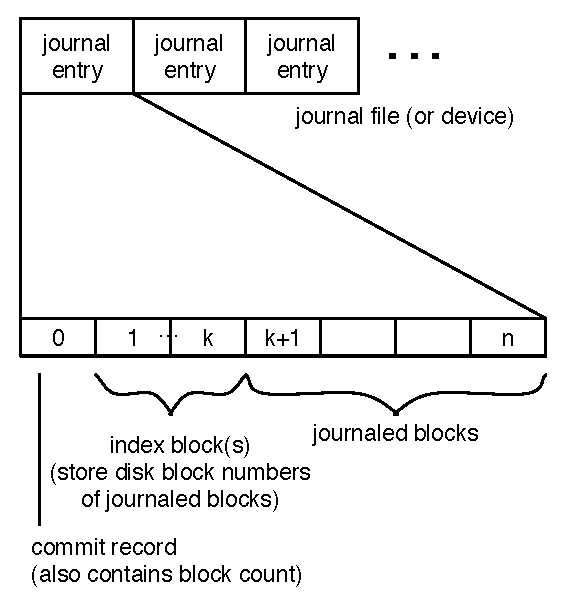
\includegraphics[width=7.5cm]{journal_diagram}
  \caption{Journal File Format}
  \label{fig:journal}
\end{center}
\end{figure}

To effect this behavior, we use two modules: a journal LFS module, and a journal
queue BD module. The function of the journal queue BD module is to hold disk
blocks that would otherwise have been written to the disk in a queue until asked
to release them. It is typically placed below the base LFS module (i.e., as that
module's BD). The journal LFS module is placed above the base LFS module, and it
knows how to construct, write, and recover the journal. Ordinarily, it keeps the
journal queue BD in a hold state, so that all file system changes are queued up.
Every so often (the ``commit interval''), it asks the journal queue BD for all
the blocks in the queue, writes them to the journal, sets up dependencies so
that the journal will be written before the disk blocks themselves, and releases
the queued blocks. This process is always guaranteed to occur at times when the
file system is in a consistent state.

Soft updates is somewhat more pervasive, because unlike full journaling, it
needs to have more information about what a file system is and what it means for
it to be ``consistent.'' Briefly, soft updates needs to guarantee that
structures on the disk are always initialized and marked as in use before they
are pointed to, and that all pointers to structures are cleared before the
structures are marked as free or reused. To accomplish this, we need the base
LFS module to help us out a little bit, by giving us ``hints'' (really, change
descriptor dependency information) as to what needs to happen before what for
each of its micro-ops. Additionally, we need those small hints to be composed
into larger hints by UHFS. These are relatively small changes to both of these
modules, and they are relatively simple to make because of how much the work is
divided up into individual LFS operations.

The write-back cache, described in section \ref{sec:solution:impl:wbcache}, then
makes sure that the changes are written in a safe order, just as it does for
journaling above. This is one of the big advantages of generalizing the write
ordering requirements of soft updates and journaling: they can share a good deal
of the more complicated code.

\subsubsection{wb\_cache}
\label{sec:solution:impl:wbcache}

In the higher levels of the system (josfs\_base, UHFS, etc) writes are
generated. The writes are arranged with dependency information that restricts
the order in which they can be written to disk. A write back cache is desirable
for performance reasons, but extreme care must be taken here because a write
back cache can reorder disk writes. It is imperative that writes from the cache
are in an order that does not violate the dependency information set up by the
higher levels.

Recall that change descriptors can reference a portion of a disk block (in fact,
they can reference as little as one bit, or as much as an entire block). The
higher levels require not that disk blocks be written in a valid order, but that
the \emph{changes} are written back in a valid order. Furthermore, we are
guaranteed that a dependency graph of changes will contain no cycles; thus it is
possible to write back the changes in order.

The cache currently is fixed size and direct mapped. When a block is read from
the cache, a reference is held to it by the cache.

If a block is written to an empty slot, a reference is held. If a block is
written over a previous version of the block, the change descriptors of the
block being written are applied to the block in the cache. If the block being
written has no slot in the cache, a block must be evicted to make room for it.

A block that needs to be evicted must be written to a lower level (currently we
mandate this to go to stable storage, not another cache), but this write may
depend on other blocks being written first. To decide how to write out the
blocks, a directed acyclic graph of changes is obtained from depman. The root of
this graph is a special ``no-op'' change descriptor that points to all of the
changes in the block that need to be written. These changes then point to other
changes, and so on.

The maximum hop distance from each change descriptor to the root change
descriptor is calculated. The write back cache then writes each leaf change to
disk. For each block that needs to be written out, if there are other changes on
the block that cannot be written (because they have dependencies on another
block), these change descriptors are ``rolled back.'' This causes the changes to
be temporarily undone. The block can then be written, and only the non-rolled
back changes will be written out. Then those change descriptors are ``rolled
forward.'' Thus, we have the capability to write out data atomically in smaller
units than whole blocks.

Note that a change descriptor may depend on a change descriptor in another write
back cache (imagine an external journal with a separate write back cache). If
this is the case, we simply tell that cache to write out the change descriptor
(with its sync() function), rather than having this cache write it itself.

Once a change has been written to the lower level, it is marked as satisfied and
removed from the graph of changes that need to be written to the disk. The cache
then finds the next chdesc furthest from the root change descriptor and writes
it to disk in the same way, and so on. Once all changes have been written to
disk, the block we wish to evict will be fully written to disk.

One may notice that this algorithm, while simple, is not optimal. That is, it
does not necessarily result in the minimal number of block writes from the write
back cache. In our usage with typical file system operations, however, we have
found that the graphs which cause non-optimal behavior do not tend to arise and
this algorithm generally gives the optimal solution.

The current write back cache has a caveat: write back caches cannot be stacked.
Intuitively, this makes sense: when writing out many change descriptors, we want
to make sure some changes are written out to stable storage before writing out
other (dependent) changes. If the change descriptors are not going straight to
disk when they are written, then what is the purpose of carefully managing the
dependencies? The next lower level will also have to be responsible for ordering
them properly before they are written to disk. More concretely, we run into a
problem with change descriptor dependencies. If we write out a change from the
write back cache to a lower level, we then expect changes that depended on that
to be able to be written now. However, these changes still cannot be written out
because their dependencies have not been satisfied. In the end, this problem
boils down to the assumption that when changes are written out from the write
back cache, they will hit stable storage.

\subsubsection{RAID}
\label{sec:solution:impl:raid}

The mirror\_bd module implements RAID 1 using two block devices. It connects two
BD interfaces together and presents a single BD interface to the layer above.
During normal operation, reads alternate between the two underlying block
devices based on the stripe size set at configuration time. Write and sync
operations are duplicated, once for each block device.

In the case where a BD operation fails, the mirror\_bd module will mark the
device as failed and switch to degraded mode. There is also a userspace tool,
mirror, to explicitly fail a device using the online configuration facility. In
degraded mode, the RAID module acts as a pass-through for the working device.
However, mirror\_bd will never fail both devices at the same time. To make BD
failures possible for disks, we enhanced the ide\_pio\_bd module so operations
time out instead of polling forever. With the mirror\_bd device in degraded
mode, users can add a block device to the raid module and return to normal mode.
The RAID module will take any module that exports a BD interface, as long as it
has the same block size and is sufficiently large. Upon device addition, the
RAID module will sync the two block devices.

mirror\_bd has some creative uses as well. One possibility is to start with
mirror\_bd in degraded mode, in place of just a disk. While the system is
running, it is then possible to add a second block device into mirror\_bd.
After the block devices are synchronized, the original disk can be safely
removed. This effectively implements disk hot swapping, as inspired by GEOM
(\S~\ref{sec:related:geom}).

\subsubsection{Loop Device}
\label{sec:solution:impl:loop}

The loop device provides a BD interface to an LFS file. Through change
descriptors and the LFS interface, the loop device is able to easily pass
dependency information to the underlying file system, preserving soft updates
and journaling dependencies. To write or sync a block, the loop device sets the
block's BD pointer and block number for use by the LFS's underlying BD, makes
the appropriate LFS call, reverts its changes to the block, and returns.

\subsubsection{Network Block Device}
\label{sec:solution:impl:nbd}

The network block device is extremely simple. It uses a straightforward
serialization of the BD interface over a TCP connection. During initialization,
it receives the block size and number of blocks from the server. For each read
request, it sends a read command and a block number to the server, and waits for
the block to be returned. For a write request, it sends a write command, block
number, and the block data. Both the client and server (which can run on either
a POSIX system or KudOS itself) required only a few hours to develop and test,
and they fit right into the rest of the system like any other block device.

\subsubsection{Online Configuration}
\label{sec:solution:impl:online}

The modman component is central to most online configuration and introspection,
providing existence, usage, configuration, and status information for CFS, LFS,
and BD module instances. Each module instance registers/unregisters itself with
modman at creation/destruction time and registers/unregisters module instance
usage. modman stores this information to respond to others' queries.

KFS RPC is implemented very much like CFS RPC: a serialized KFS is used to
communicate between KFS server and clients via KudOS IPC message passing.  Each
KFS function is reimplemented as an RPC stub, allowing an object file to be
linked to either the KFS IPC client or server library. Client programs are thus
able to reconfigure the kfsd environment using the same functions that would be
used within kfsd.

The kfsgraph program uses KFS RPC to construct a module usage graph, showing
existing module instances, which instances use which others, and instances'
configuration and status. kfsgraph can output this graph to text or to AT\&T's
graphviz dot format. Section~\ref{sec:eval} shows examples of kfsgraph's output.

The programs mount and umount, named for their similarity to the Unix tools of
the same names, provide a general case, easy to use configuration interface.
Given a BD type of IDE, nbd, loop, or an existing BD and a mount point, mount
constructs the given base BD, caches and block resizers as appropriate, a
josfs\_base or wholedisk as appropriate, UHFS, and connects these to the table
classifier at the given mount point. mount optionally allows specification of
whether journaling is to be used (and if so, where to journal to), whether to
fsck the file system, how large a cache to use, and whether to use a write back
or write through cache. umount takes a mount point and destructs all modules
down the chain that are no longer in use.
